\section{System Implementation: User Interface and Backend Architecture}

This section presents the implementation of the user-facing components of the Amal platform, including the web application, mobile application, and backend API server. These components serve as the bridge between end-users and the underlying AI models, providing accessible interfaces for drug addiction support services.

\subsection{System Architecture Overview}

The Amal platform follows a client-server architecture with clear separation of concerns. Figure~\ref{fig:architecture} illustrates the overall system design, comprising three main layers: (1) presentation layer (web and mobile clients), (2) application layer (API server and orchestrator), and (3) AI layer (intent classification, RAG, and support models).

\begin{figure}[h]
\centering
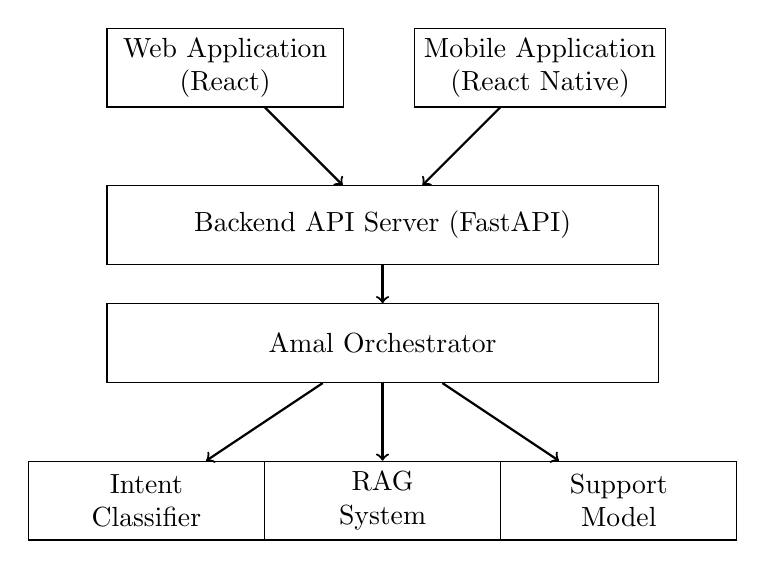
\begin{tikzpicture}[
    box/.style={rectangle, draw, minimum width=3cm, minimum height=1cm, align=center},
    arrow/.style={->, thick}
]
% Presentation Layer
\node[box] (web) at (0,4) {Web Application\\(React)};
\node[box] (mobile) at (4,4) {Mobile Application\\(React Native)};

% Application Layer
\node[box, minimum width=7cm] (api) at (2,2) {Backend API Server (FastAPI)};
\node[box, minimum width=7cm] (orch) at (2,0.5) {Amal Orchestrator};

% AI Layer
\node[box] (intent) at (-1,-1.5) {Intent\\Classifier};
\node[box] (rag) at (2,-1.5) {RAG\\System};
\node[box] (support) at (5,-1.5) {Support\\Model};

% Arrows
\draw[arrow] (web) -- (api);
\draw[arrow] (mobile) -- (api);
\draw[arrow] (api) -- (orch);
\draw[arrow] (orch) -- (intent);
\draw[arrow] (orch) -- (rag);
\draw[arrow] (orch) -- (support);
\end{tikzpicture}
\caption{Amal Platform Architecture}
\label{fig:architecture}
\end{figure}

\subsection{Backend API Server}

\subsubsection{Technology Selection}

The backend server was implemented using FastAPI~\cite{fastapi}, a modern Python web framework. FastAPI was selected based on the following criteria:

\begin{enumerate}
    \item \textbf{Performance}: FastAPI achieves performance comparable to Node.js and Go, handling over 30,000 requests per second in benchmarks. This is critical for real-time AI inference applications.
    
    \item \textbf{Asynchronous Support}: Native async/await support enables efficient handling of concurrent requests, particularly important when multiple users simultaneously query AI models.
    
    \item \textbf{Type Safety}: Integration with Pydantic provides automatic request validation and serialization, reducing runtime errors and improving API reliability.
    
    \item \textbf{ML Ecosystem Compatibility}: Seamless integration with PyTorch, Transformers, and other machine learning libraries used by the AI models.
    
    \item \textbf{Automatic Documentation}: OpenAPI (Swagger) documentation is generated automatically, facilitating frontend development and API testing.
\end{enumerate}

\subsubsection{API Design}

The REST API exposes endpoints for chat functionality and user authentication. Table~\ref{tab:endpoints} summarizes the available endpoints.

\begin{table}[h]
\centering
\caption{API Endpoints}
\label{tab:endpoints}
\begin{tabular}{@{}llp{6cm}@{}}
\toprule
Endpoint & Method & Description \\
\midrule
\texttt{/chat} & POST & Process user message through AI pipeline \\
\texttt{/health} & GET & Server health and model status check \\
\texttt{/auth/signup} & POST & User registration \\
\texttt{/auth/login} & POST & User authentication \\
\texttt{/auth/forgot-password} & POST & Password reset request \\
\texttt{/auth/reset-password} & POST & Password reset with token \\
\texttt{/auth/refresh} & POST & Access token refresh \\
\texttt{/auth/me} & GET & Current user information \\
\bottomrule
\end{tabular}
\end{table}

\subsubsection{Orchestrator Pattern}

The core of the backend is the \texttt{AmalBackend} orchestrator class, which coordinates the flow between AI models. Algorithm~\ref{alg:orchestrator} describes the query processing pipeline.

\begin{algorithm}[h]
\caption{Query Processing Pipeline}
\label{alg:orchestrator}
\begin{algorithmic}[1]
\REQUIRE User query $q$
\ENSURE Response $r$, intent $i$, language $l$
\STATE $l \leftarrow \text{DetectLanguage}(q)$
\STATE $i, c \leftarrow \text{IntentClassifier.predict}(q)$
\IF{$i = \text{``Out of context''}$}
    \STATE $r \leftarrow \text{GetLocalizedRejection}(l)$
\ELSIF{$i = \text{``Harm''}$}
    \STATE $r \leftarrow \text{GetCrisisResponse}(l)$ \COMMENT{Includes 3033 hotline}
\ELSIF{$i = \text{``Exact fact''}$}
    \STATE $r \leftarrow \text{RAGBackend.generate}(q, l)$
\ELSIF{$i = \text{``Looking for support''}$}
    \STATE $r \leftarrow \text{SupportModel.generate}(q)$
\ENDIF
\RETURN $r, i, l$
\end{algorithmic}
\end{algorithm}

\subsubsection{Language Detection}

Given the multilingual nature of the target population, the system implements automatic language detection supporting Arabic, French, Darija (Algerian Arabic), and English. The detection algorithm analyzes the ratio of Arabic to Latin characters:

\begin{equation}
\text{lang} = 
\begin{cases}
\text{ar} & \text{if } \frac{|\text{Arabic chars}|}{|\text{Total chars}|} > 0.7 \\
\text{dz} & \text{if } 0.3 \leq \frac{|\text{Arabic chars}|}{|\text{Total chars}|} \leq 0.7 \\
\text{fr/en} & \text{otherwise (determined by lexical analysis)}
\end{cases}
\end{equation}

\subsubsection{Authentication System}

The authentication system implements JSON Web Tokens (JWT) for stateless authentication, suitable for both web and mobile clients. Key security features include:

\begin{itemize}
    \item Password hashing using SHA-256 with random salt
    \item Access tokens with 24-hour expiration
    \item Refresh tokens with 30-day expiration for seamless re-authentication
    \item Token rotation on refresh to prevent replay attacks
\end{itemize}

The system implements a ``lazy login'' pattern where users can access the chat functionality without authentication, reducing friction for users seeking immediate help. Authentication is optional and enables data synchronization across devices.

\subsection{Web Application}

\subsubsection{Technology Stack}

The web application was developed using React 18~\cite{react} with TypeScript for type safety. Table~\ref{tab:web-stack} presents the complete technology stack.

\begin{table}[h]
\centering
\caption{Web Application Technology Stack}
\label{tab:web-stack}
\begin{tabular}{@{}lll@{}}
\toprule
Technology & Version & Purpose \\
\midrule
React & 18.2 & User interface library \\
TypeScript & 5.2 & Static typing \\
Vite & 5.0 & Build tool and development server \\
Tailwind CSS & 3.3 & Utility-first styling \\
React Router & 6.20 & Client-side routing \\
Zustand & 4.4 & State management \\
Lucide React & 0.294 & Icon library \\
\bottomrule
\end{tabular}
\end{table}

\subsubsection{Framework Justification}

\paragraph{React} was selected for its component-based architecture enabling modular, reusable code. The virtual DOM efficiently updates only changed elements, crucial for the real-time chat interface. React's extensive ecosystem provides mature solutions for routing, state management, and internationalization.

\paragraph{Vite} was chosen over Create React App for its superior development experience. Vite leverages native ES modules for instant server startup (under 300ms) and hot module replacement under 50ms, significantly improving developer productivity.

\paragraph{Tailwind CSS} enables rapid UI development through utility classes while maintaining design consistency. The framework's built-in support for RTL layouts (via \texttt{rtl:} variants) and dark mode (\texttt{dark:} variants) simplified multilingual and accessibility implementation.

\paragraph{Zustand} provides lightweight state management with minimal boilerplate. At 1.1KB gzipped (compared to Redux's 7KB+), it reduces bundle size while offering excellent TypeScript integration and built-in persistence middleware.

\subsubsection{Application Structure}

The application follows a feature-based architecture:

\begin{verbatim}
src/
├── components/          # Shared UI components
│   └── navigation/      # Navbar, Footer
├── features/            # Feature modules
│   ├── auth/           # Authentication
│   ├── chat/           # AI chat interface
│   ├── home/           # Landing page
│   └── resources/      # Educational content
├── services/           # API communication
└── store/              # Global state
\end{verbatim}

This structure ensures separation of concerns, with each feature encapsulating its own pages, components, and state management.

\subsubsection{Multilingual and RTL Support}

The application supports four languages with full right-to-left (RTL) layout for Arabic scripts. Language switching dynamically updates:

\begin{itemize}
    \item Document direction (\texttt{dir="rtl"} or \texttt{dir="ltr"})
    \item Text alignment and component layouts
    \item Localized content and error messages
\end{itemize}

\subsubsection{Chat Interface Implementation}

The chat interface provides real-time communication with the AI backend. Key implementation details include:

\begin{itemize}
    \item Optimistic UI updates for immediate user feedback
    \item Message streaming support for long responses
    \item Automatic scroll management for new messages
    \item Loading states and error handling with retry capability
\end{itemize}

\subsection{Mobile Application}

\subsubsection{Technology Selection}

The mobile application was developed using React Native~\cite{reactnative} with Expo SDK 52. This approach enables cross-platform deployment from a single codebase.

\begin{table}[h]
\centering
\caption{Mobile Application Technology Stack}
\label{tab:mobile-stack}
\begin{tabular}{@{}lll@{}}
\toprule
Technology & Version & Purpose \\
\midrule
React Native & 0.76 & Cross-platform framework \\
Expo & SDK 52 & Development platform \\
TypeScript & 5.3 & Static typing \\
React Navigation & 7.x & Native navigation \\
Zustand & 4.4 & State management \\
AsyncStorage & 1.23 & Local data persistence \\
\bottomrule
\end{tabular}
\end{table}

\subsubsection{Cross-Platform Justification}

React Native was selected over native development (Swift/Kotlin) and alternative frameworks (Flutter, Ionic) based on:

\begin{enumerate}
    \item \textbf{Code Sharing}: Approximately 90\% code sharing between Android and iOS reduces development time by 40-50\%.
    
    \item \textbf{Native Performance}: Unlike hybrid frameworks, React Native compiles to native components, providing near-native performance.
    
    \item \textbf{Ecosystem Synergy}: Shared knowledge and libraries with the React web application accelerates development.
    
    \item \textbf{Expo Platform}: Expo eliminates native build configuration complexity, enabling rapid prototyping and over-the-air updates.
\end{enumerate}

\subsubsection{Navigation Architecture}

The application implements a bottom tab navigation pattern with five main screens:

\begin{enumerate}
    \item \textbf{Home}: Landing screen with quick actions and crisis hotline
    \item \textbf{Chat}: AI conversation interface
    \item \textbf{Resources}: Educational content and treatment centers
    \item \textbf{Settings}: Language, theme, and account preferences
    \item \textbf{Auth}: Login, signup, and password recovery
\end{enumerate}

React Navigation 7 provides native navigation primitives on each platform, ensuring platform-appropriate animations and gestures.

\subsubsection{State Persistence}

User preferences and authentication tokens are persisted using AsyncStorage with Zustand middleware:

\begin{lstlisting}[language=JavaScript, caption=Persistent State Configuration]
export const useAuthStore = create(
  persist(
    (set) => ({
      user: null,
      accessToken: null,
      // ... actions
    }),
    {
      name: 'amal-auth',
      storage: createJSONStorage(() => AsyncStorage),
    }
  )
);
\end{lstlisting}

This ensures users remain authenticated across app restarts and enables offline access to cached data.

\subsubsection{API Integration}

The mobile application communicates with the backend via REST API. For physical device testing, the API URL must reference the development machine's IP address rather than localhost:

\begin{lstlisting}[language=JavaScript, caption=API Configuration]
// For physical device testing
const API_BASE_URL = 'http://192.168.x.x:8000';

// For Android emulator
const API_BASE_URL = 'http://10.0.2.2:8000';
\end{lstlisting}

\subsection{User Interface Design Considerations}

\subsubsection{Target Audience}

The interface was designed for users aged 20-60 in Algeria, requiring:

\begin{itemize}
    \item Professional, non-stigmatizing visual design
    \item Clear typography with adequate contrast ratios
    \item Intuitive navigation without complex interactions
    \item Prominent display of crisis hotline (3033)
\end{itemize}

\subsubsection{Accessibility}

Both applications implement accessibility best practices:

\begin{itemize}
    \item Semantic HTML elements and ARIA labels
    \item Keyboard navigation support (web)
    \item Screen reader compatibility
    \item Minimum touch target sizes of 44x44 points (mobile)
    \item Color contrast ratios meeting WCAG 2.1 AA standards
\end{itemize}

\subsubsection{Dark Mode}

Both applications support dark and light themes, persisted in user preferences. Theme switching is implemented via CSS custom properties (web) and React Native's appearance API (mobile).

\subsection{Performance Optimization}

\subsubsection{Web Application}

\begin{itemize}
    \item \textbf{Code Splitting}: Vite automatically splits code by route, loading only necessary JavaScript
    \item \textbf{CSS Purging}: Tailwind removes unused styles, reducing CSS payload by over 95\%
    \item \textbf{Asset Optimization}: Images compressed and served in modern formats (WebP)
\end{itemize}

\subsubsection{Mobile Application}

\begin{itemize}
    \item \textbf{FlatList Virtualization}: Chat messages rendered using virtualized lists for memory efficiency
    \item \textbf{Memoization}: React.memo prevents unnecessary re-renders of static components
    \item \textbf{Lazy Loading}: Screens loaded on-demand to reduce initial bundle size
\end{itemize}

\subsubsection{Backend}

\begin{itemize}
    \item \textbf{Model Preloading}: AI models loaded at server startup to eliminate cold-start latency
    \item \textbf{Async Processing}: Non-blocking request handling for concurrent users
    \item \textbf{CORS Configuration}: Optimized headers for cross-origin requests
\end{itemize}

\subsection{Deployment Considerations}

The system is designed for containerized deployment:

\begin{itemize}
    \item \textbf{Backend}: Docker container with Python 3.10, GPU support via NVIDIA Container Toolkit
    \item \textbf{Frontend}: Static files served via Nginx or CDN
    \item \textbf{Mobile}: Distribution via Google Play Store and Apple App Store, with Expo EAS Build
\end{itemize}

\subsection{Summary}

This section presented the implementation of the Amal platform's user-facing components. The web application, built with React and TypeScript, provides a responsive, multilingual interface accessible from any modern browser. The mobile application, developed with React Native and Expo, extends accessibility to smartphone users across Android and iOS platforms. The FastAPI backend serves as the integration layer, orchestrating AI model inference while providing secure authentication and efficient request handling. Together, these components deliver a cohesive user experience for drug addiction support services in Algeria.

% References for this section
\begin{thebibliography}{9}
\bibitem{fastapi}
Ramírez, S. (2018). FastAPI. \url{https://fastapi.tiangolo.com}

\bibitem{react}
Meta Platforms, Inc. (2023). React: A JavaScript library for building user interfaces. \url{https://react.dev}

\bibitem{reactnative}
Meta Platforms, Inc. (2023). React Native: Learn once, write anywhere. \url{https://reactnative.dev}
\end{thebibliography}
